\documentclass[../main.text]{subfiles}
\begin{document}
\subsection{Quantitative}

While clustering (~\ref{sec:cluster}) techniques are very effective for understanding large datasets, often a researcher explicitly wants to explore the relationship between individual observations. Visualizations that emphasize observational relationships often either group like observations together or explore pairwise interactions. 


\subsubsection{Stacked Plot}
\label{sec:stacked}
\begin{figure}[H]
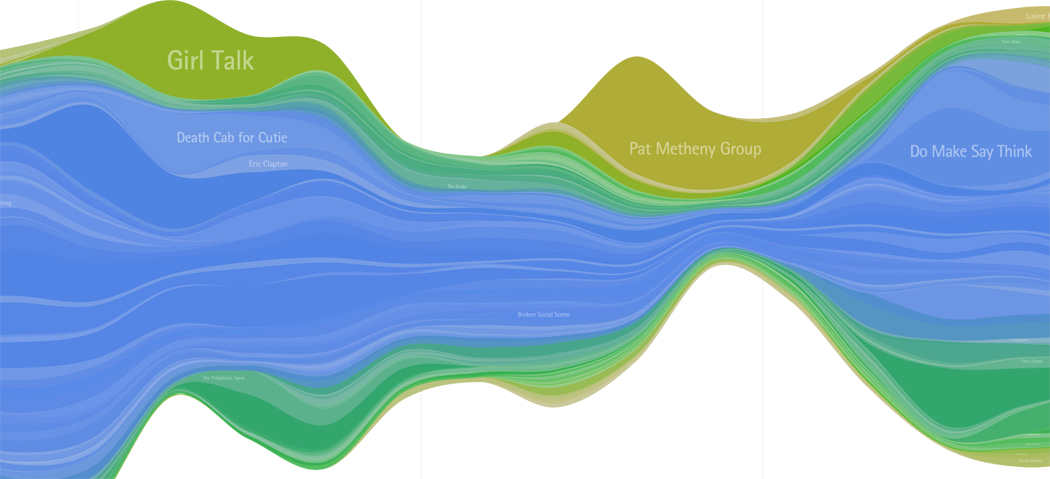
\includegraphics[width=\textwidth]{stream.png}
\caption{Section of graphic designer Lee Byron's \textit{Listening History} \cite{fry_what_????,l._byron_stacked_2008} project based on last.fm data. The spikes in listening to new artists following periods of decreased listening suggest a possible dependency between previous listening behavior and openness to trying new music. The figure is from \textit{Stacked Graphs-Geometry \& Aesthetics} \cite{l._byron_stacked_2008}
}
\label{fig:streamgraph}
\end{figure}

For timeseries, or other continuous functional data, a streamgraph shows how categories of data change across the time \textit{component} of the visualization. A stream graph, which is a type of stacked graph, is created by either horizontally or vertically stacking continuous data \cite{Heer:2010:TTV:1743546.1743567, l._byron_stacked_2008}. In \textit{Listening History} \cite{fry_what_????,l._byron_stacked_2008}, Lee Byron encodes each artist as a unique color, but groups the colors such that more established authors are represented by cooler colors (blues) and newer artists by warmer colors (yellows). In figure~\ref{fig:streamgraph}, the more established artists maintain a stable listener base over time, while newer artists wax and wane in popularity. Figure~\ref{fig:streamgraph} shows a seasonal pattern of fairly consistent listening over the year and a severe acute drop in listening in December, after which follows a spike in popularity for the then new artist \textit{DJ Shadow}. A drop in mid-July leads to a spike for the new bands \textit{Pat Metherly Group} and \textit{Prefuse73}. This suggests a conditional dependency between low periods of listening and choosing to listen to new acts. A stacked graph can be used to infer conditional dependency when encoded in such a way that it can provide information on two or more variables, but the graph is limited to about 3 or 4 variables. 


\subsubsection{Parallel Coordinates}
\label{sec:pcp}
\begin{figure}{H}
  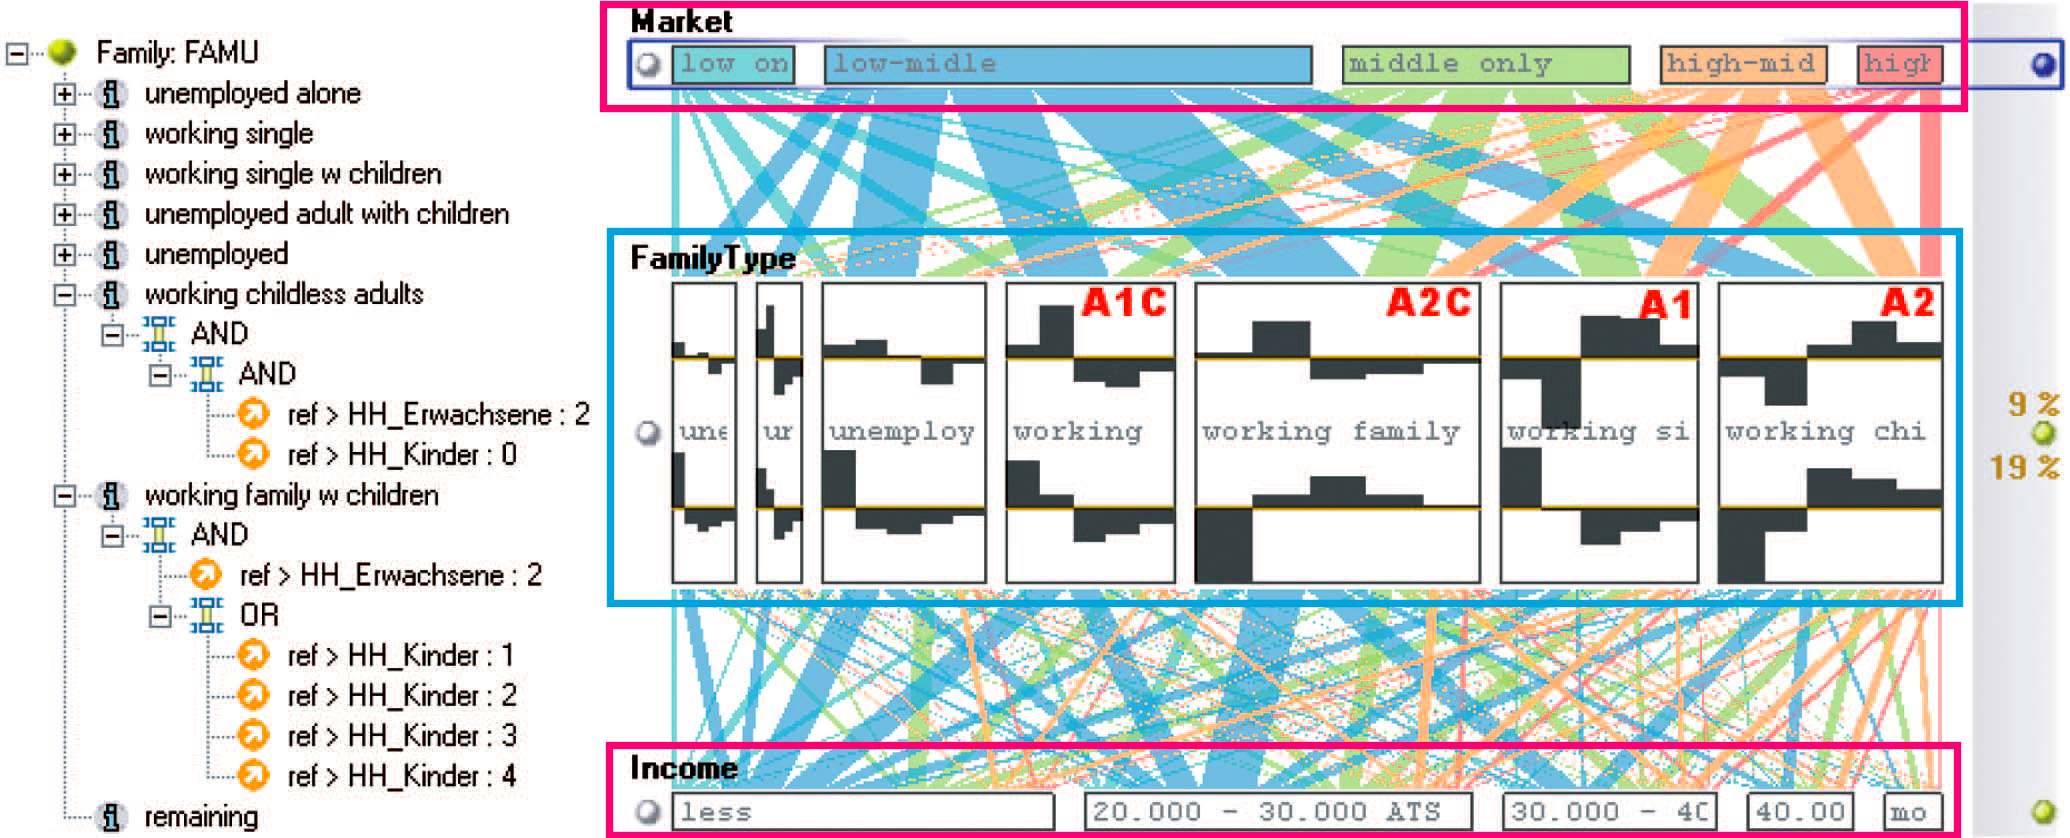
\includegraphics[width=\textwidth]{parallelsets.png}
  \caption{On the left is the categorical view where users can select a set of interest, for example a working family with one or more children. At the top of the parallel sets graphs is a set of supermarket categories. The width of the lines flowing out of each category is representational of the number of elements that are in both that category and the category the line is going into. The left most line is representational of the number of households that shop at a low-end supermarket and that have a family type of unemployed. The top histograms show how each family type is distributed across all market types, and the bottom histograms show how each family type is distribute across income levels. Like the lines going into the family type view, the width of the lines represents the number of households of that family type in that income level and are color coded by supermarket type. Because it provides a filtering tool, parallel sets can be used to query whether supermarket and income are conditionally dependent on categorical subsets of family types. This figure is taken from \textit{Parallel sets: Interactive exploration and visual analysis of categorical data} \cite{kosara_parallel_2006}}
  \label{fig:parallelsets}
\end{figure}

When there are no key semantics to preserve, one method for showing conditional dependence is to combine the pairwise visualizations of a parallel coordinates plot with histograms and categorical filtering. The Parallel Sets tool shown in figure~\ref{fig:parallelsets} is explicitly designed to show frequencies
of set membership in hierarchal ordered categorical sets \cite{kosara_parallel_2006}. Similarly to the flexible linked axis version of the parallel coordinates plot \cite{claessen_flexible_2011}, Parallel Sets explicitly groups observations by category and shows how the set of observations in those categories flows into another set of categories. Parallel sets treats each categorical set independently, but indicates conditional dependency through cross tables and by grouping the data. This is indicated via color and is based on an active subcategory that then becomes the grouping variable for the cross tables. In Parallel Sets, quantitative data is converted to categorical data via binning. Parallel Sets provides a filtering interface for users to test out how different subsets of family type affect family income or choice of supermarket, which in turn can be used to explore whether there is a conditional dependency amongst these variables. The many-to-many parallel coordinate plot is another type of generalized parallel coordinates where all possible pairs are explored \cite{lind_many--many_2009}. Parallel sets is particularly good for visualizing datasets where the conditional dependency is on categorical datasets, but like many of the other techniques is limited to a relatively small number of variables. 

\subsubsection{Partial Dependency}
\label{sec:pdp}

\begin{figure}[H]
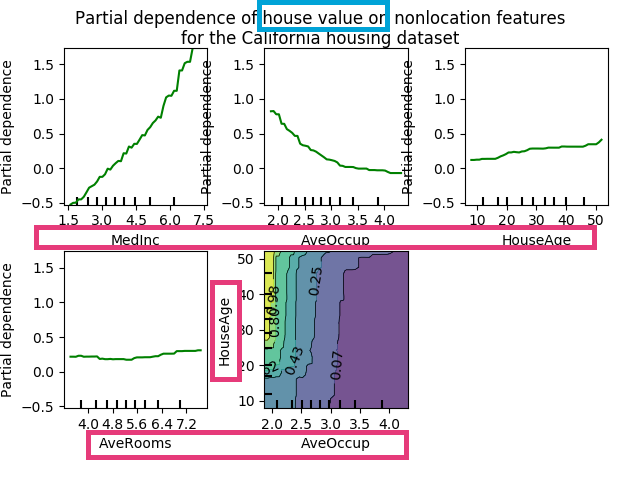
\includegraphics[width=1\textwidth]{partial_dependence}
\caption{Taken from \textit{Scikit Learn} \cite{_partial_????}, the line plots show that California housing prices are partially dependent on occupancy and median income. The heatmap shows that housing prices rise for old houses, but only if the house does not have many occupants.}
\label{fig:partialdependence}
\end{figure}

While Streamgraphs (\ref{sec:stacked}) require a continuous variable and Parallel Sets (\ref{sec:pcp} require categorical variables, the partial dependency plot is designed for quantitative observations. One way to show dependencies is to plot one variable against another, but those methods often do not measure the joint effect of the variables in the dataset. One way to analyze this interaction in the California Housing dataset is to use a regression method \cite{_elements_2009,scikit-learn} to measure the partial dependence. As shown in figure~\ref{fig:partialdependence}, the 4 one-way partial dependence line plots and the two-way partial dependence heatmap show how California housing prices are marginally dependent on median income, average occupancy and slightly on the age of the house. While marginal dependence is not conditional dependence, it establishes that there is a probabilistic relationship between housing prices and median income, average number of occupants, and the age of the house. These variables are then explored further in the heatmap, which pinpoints that the marginal probabilities between house age and occupancy are for older houses with few people. Because a house can not get younger, it can be inferred that price is partially dependent on age. In effect, partial dependence plots are computing partial conditional dependencies since they show the probabilistic dependence between a target function and a set of target features. The target features are any set of discrete observations, and the target function is a modeling of a continuous observation. While flexible in terms of what data it can be used with, partial dependence plots are limited in scope to datasets and questions that can be framed as regression problems. 
\end{document}